\subsection{Relativistisches Coulombproblem} 
	\begin{align*}
		H &= c \vec{\alpha} \cdot \vec{p} + \beta m c^2 + V(r) ,&
		V(r) &= -\frac{Z e^2}{4 \pi r} = - \frac{Z \alpha \hbar c}{r} 
	\end{align*}
	\begin{align*}
		(c \vec{\alpha} \vec{p} + \beta m c^2) \psi &= (E-V)\psi \\
		(c \vec{\alpha} \vec{p} + \beta m c^2)^2 \psi &= (c \vec{\alpha} \vec{p} +\beta m c^2)(E-V) \psi \\
		pV \psi = \frac{\hbar}{i} \vec{\nabla} (V \psi) &=
		\frac{\hbar}{i} V \vec{\nabla} \psi + \frac{\hbar}{i} \psi (\vec{\nabla} V)\\
		(c^2 \vec{p}^2 + m^2 c^4) \psi 
		&= \left[(E-V)^2 + \frac{\hbar c}{i} \vec{\alpha} (\vec{\nabla} V)\right] \psi
	\end{align*}
	\begin{align*}
		\Rightarrow \left\{
			\vec{p}^2 + \frac{i\hbar}{c} \vec{\alpha} (\vec{\nabla} V) 
			- \frac{(E-V)^2}{c^2} + m^2c^2
		\right\} \psi &= 0 \\
		p^2 = p_r^2 + \frac{1}{r^2} \vec{L}^2 =
		-\hbar^2 \frac{1}{r} \frac{\partial^2}{\partial r^2} r + \frac{1}{r^2} \vec{L}^2 \\
		\left\{
			-\hbar^2 \frac{1}{r} \frac{\partial^2}{\partial r^2} r +
			\frac{1}{r^2} \vec{L}^2 - \frac{i Z \alpha \hbar^2}{r^3} \vec{\alpha}\cdot \vec{r}
			- \frac{2Z\alpha E \hbar}{cr} - \frac{E^2}{c^2} + m^2c^2
		\right\}  \psi &= 0
	\end{align*}
Problem $\frac{\vec{\alpha} \cdot \vec{r}}{r^3}$-Term 

Temple-Operator: \marginpar{07.12.15}
	\begin{align*}
		\Lambda &= -\frac{1}{\hbar} (2 \vec{L} \cdot \vec{S} + \hbar^2) 
		- \frac{i Z \alpha \hbar}{r} \vec{\alpha} \cdot \vec{r} \\
		\Lambda^2 &= \vec{L}^2 + 2 \vec{L} \cdot \vec{S} + \hbar^2
		- Z^2 \alpha^2 \hbar^2 & &\text{(Rechnung)} \\
		\Lambda (\Lambda + \hbar) &= \Lambda^2 + \Lambda \hbar =
		\vec{L}^2 - \frac{i Z \alpha \hbar^2}{r} \vec{\alpha} \cdot \vec{r}
		- Z^2 \alpha^2 \hbar^2
	\end{align*}
	\begin{align*}
		\Rightarrow \underbrace{ \left(
				-\hbar^2 \frac{1}{r} \frac{\partial^2}{\partial r^2} r 
				+ \frac{1}{r^2} \Lambda (\Lambda + \hbar) 
				-\frac{2Z\alpha \hbar E}{cr} -\frac{E^2}{c^2} + m^2c^2
			\right)}_{\mathclap{W(\vec{r})}} \psi
		&= 0
	\end{align*}
	\begin{align*}
		[\Lambda, r] &= 0 ,& \left[\Lambda, \frac{\partial}{\partial r}\right] &= 0 
		&\Rightarrow [\Lambda, W] &= 0
	\end{align*}
$\Rightarrow$ Es existiert gemeinsame Eigenbasis von $W$ und $\Lambda$.
	\begin{align*}
		\Lambda^2 &= \vec{J}^2 - \vec{S}^2 + \hbar^2 - Z^2 \alpha^2 \hbar^2 
		= \vec{J}^2 + \left(\frac{1}{4} - Z^2\alpha^2\right) \hbar^2 \\
		\Lambda^2 \psi &= 
		\left(j (j+1) + \frac{1}{4} - Z^2 \alpha^2\right) \hbar^2 \psi 
		= \underbrace{\hbar^2 \left[\left(j + \frac{1}{2}\right)^2 - Z^2 \alpha^2\right]}_{\mathclap{\lambda^2}} \psi  
	\end{align*}
$\Lambda \psi = \lambda \psi$ mit $\lambda = \pm \hbar \sqrt{\left(j + \frac{1}{2}\right) - Z^2\alpha^2}$ 
	\begin{align*}
		\Lambda(\Lambda + \hbar) \psi &= \lambda(\lambda + \hbar) \psi =
		\hbar^2 \tilde{\ell} (\tilde{\ell} + 1) \\
		&(\text{analog zu } \vec{L}^2 \psi = \ell(\ell + 1) \hbar^2 \psi, \text{ aber } \tilde{\ell} \notin \mathds{N}_0)
	\end{align*}
	\begin{align*}
		\tilde{\ell} &=
		\left\{ 
		\begin{aligned}
			\frac{\lambda}{\hbar}& ,& \lambda &> 0 \\
			-\left(\frac{\lambda}{\hbar} + 1\right)& ,& \lambda &< 0
		\end{aligned}
		\right.
		,& 
		\tilde{\ell} &> -1
	\end{align*}
	\begin{align*}
		& &\left(
			-\frac{\hbar^2}{r} \frac{\partial^2}{\partial r^2} r 
			+ \frac{\hbar^2 \tilde{\ell} (\tilde{\ell} + 1)}{r^2} 
			- \frac{2 Z \alpha \hbar E}{cr} 
			- \frac{E^2}{c^2} + m^2c^2
		\right) \psi &= 0 \\
		\text{Ähnlich wie:}& \\
		& &\left(
			-\frac{\hbar^2}{r} \frac{\partial^2}{\partial r^2} r 
			+ \frac{\hbar^2 \ell (\ell + 1)}{r^2} 
			- \frac{2 Z \alpha \hbar cm}{r} 
			- 2mE
		\right) \psi_{N\ell}&= 0
	\end{align*}
Nicht relativistisch: Coulombproblem: Wird gelöst durch $\psi_{N\ell}$ mit Eigenwerten
	\begin{align*}
		E_{N\ell} &= -\frac{1}{2n^2} mc^2 Z^2 \alpha^2 ,&
		n &= N + \ell + 1
	\end{align*}
$N$ ist die Anzahl der Knoten.

Relativistisches Coulombproblem gibt Energien:
	\begin{align*}
		\tilde{E}_{N\tilde{\ell}} &= 
		-\frac{1}{2\tilde{n}^2} \tilde{m} c^2 Z^2 \alpha^2 &\text{mit }
		\tilde{n} &= N + \tilde{\ell} + 1
	\end{align*}
Vergleich mit nicht relativistischem Problem liefert:
	\begin{align*}
		2 \tilde{m} \tilde{E} &= \frac{E^2}{c^2} -m^2 c^2 &
		\tilde{m} &= \frac{E}{c^2} \\
		\tilde{E} &= \frac{1}{2E} (E^2 - m^2 c^2) \\
		\frac{E^2 - m^2 c^4}{2E} &= -\frac{1}{2 \tilde{n}^2} Z^2 \alpha^2 E \\
		&\Rightarrow E^2 \left( 1 + \frac{Z^2 \alpha^2}{\tilde{n}^2}\right) 
		= m^2 c^4
	\end{align*}
	\begin{align*}
		E_{N \tilde{\ell}} &= \frac{mc^2}{\sqrt{1 + \frac{Z^2 \alpha^2}{\tilde{n}^2}}} \\
		n &= N + \ell + 1 = N + 1 + j \pm \frac{1}{2} \\
		\tilde{n} &= N + \tilde{\ell} + 1 = n - j \mp \frac{1}{2} + \tilde{\ell}\\
		&= \left\{
			\begin{aligned}
				n - j + \frac{\lambda}{\hbar} + \frac{1}{2} \\
				n - j - \frac{\lambda}{\hbar} - \frac{1}{2}
			\end{aligned}
		\right\} 
		= n - j - \frac{1}{2}+ \sqrt{\left(j + \frac{1}{2}\right)^2 - Z^2 \alpha^2} \\
		n &= 1, 2, 3, \ldots ~(\text{Hauptquantenzahl})
	\end{align*}
Zustände mit gleichem $j$ sind entartet, da $\tilde{n}$ nur von $n$ und $j$, nicht aber von $\ell$ abhängt.
	\begin{align*}
		E_{nj} &= \frac{mc^2}{\sqrt{1 + Z^2 \alpha^2 \left(n - j -\frac{1}{2} + \sqrt{\left(j + \frac{1}{2}\right)^2 - Z^2 \alpha^2}\right)^{-2}}} \\
		&= mc^2 - \frac{Z^2 \alpha^2 m c^2}{2 n^2} + \mathscr{O} ((Z\alpha)^2)
	\end{align*}
$>0$, weil $E_{nj}$ $mc^2$ beinhält
	\begin{align*}
		E_{nj} - mc^2 &< 0 & &\text{(Bindungsenergie)}
	\end{align*}
	\begin{figure*} [h]
		\begin{center}
			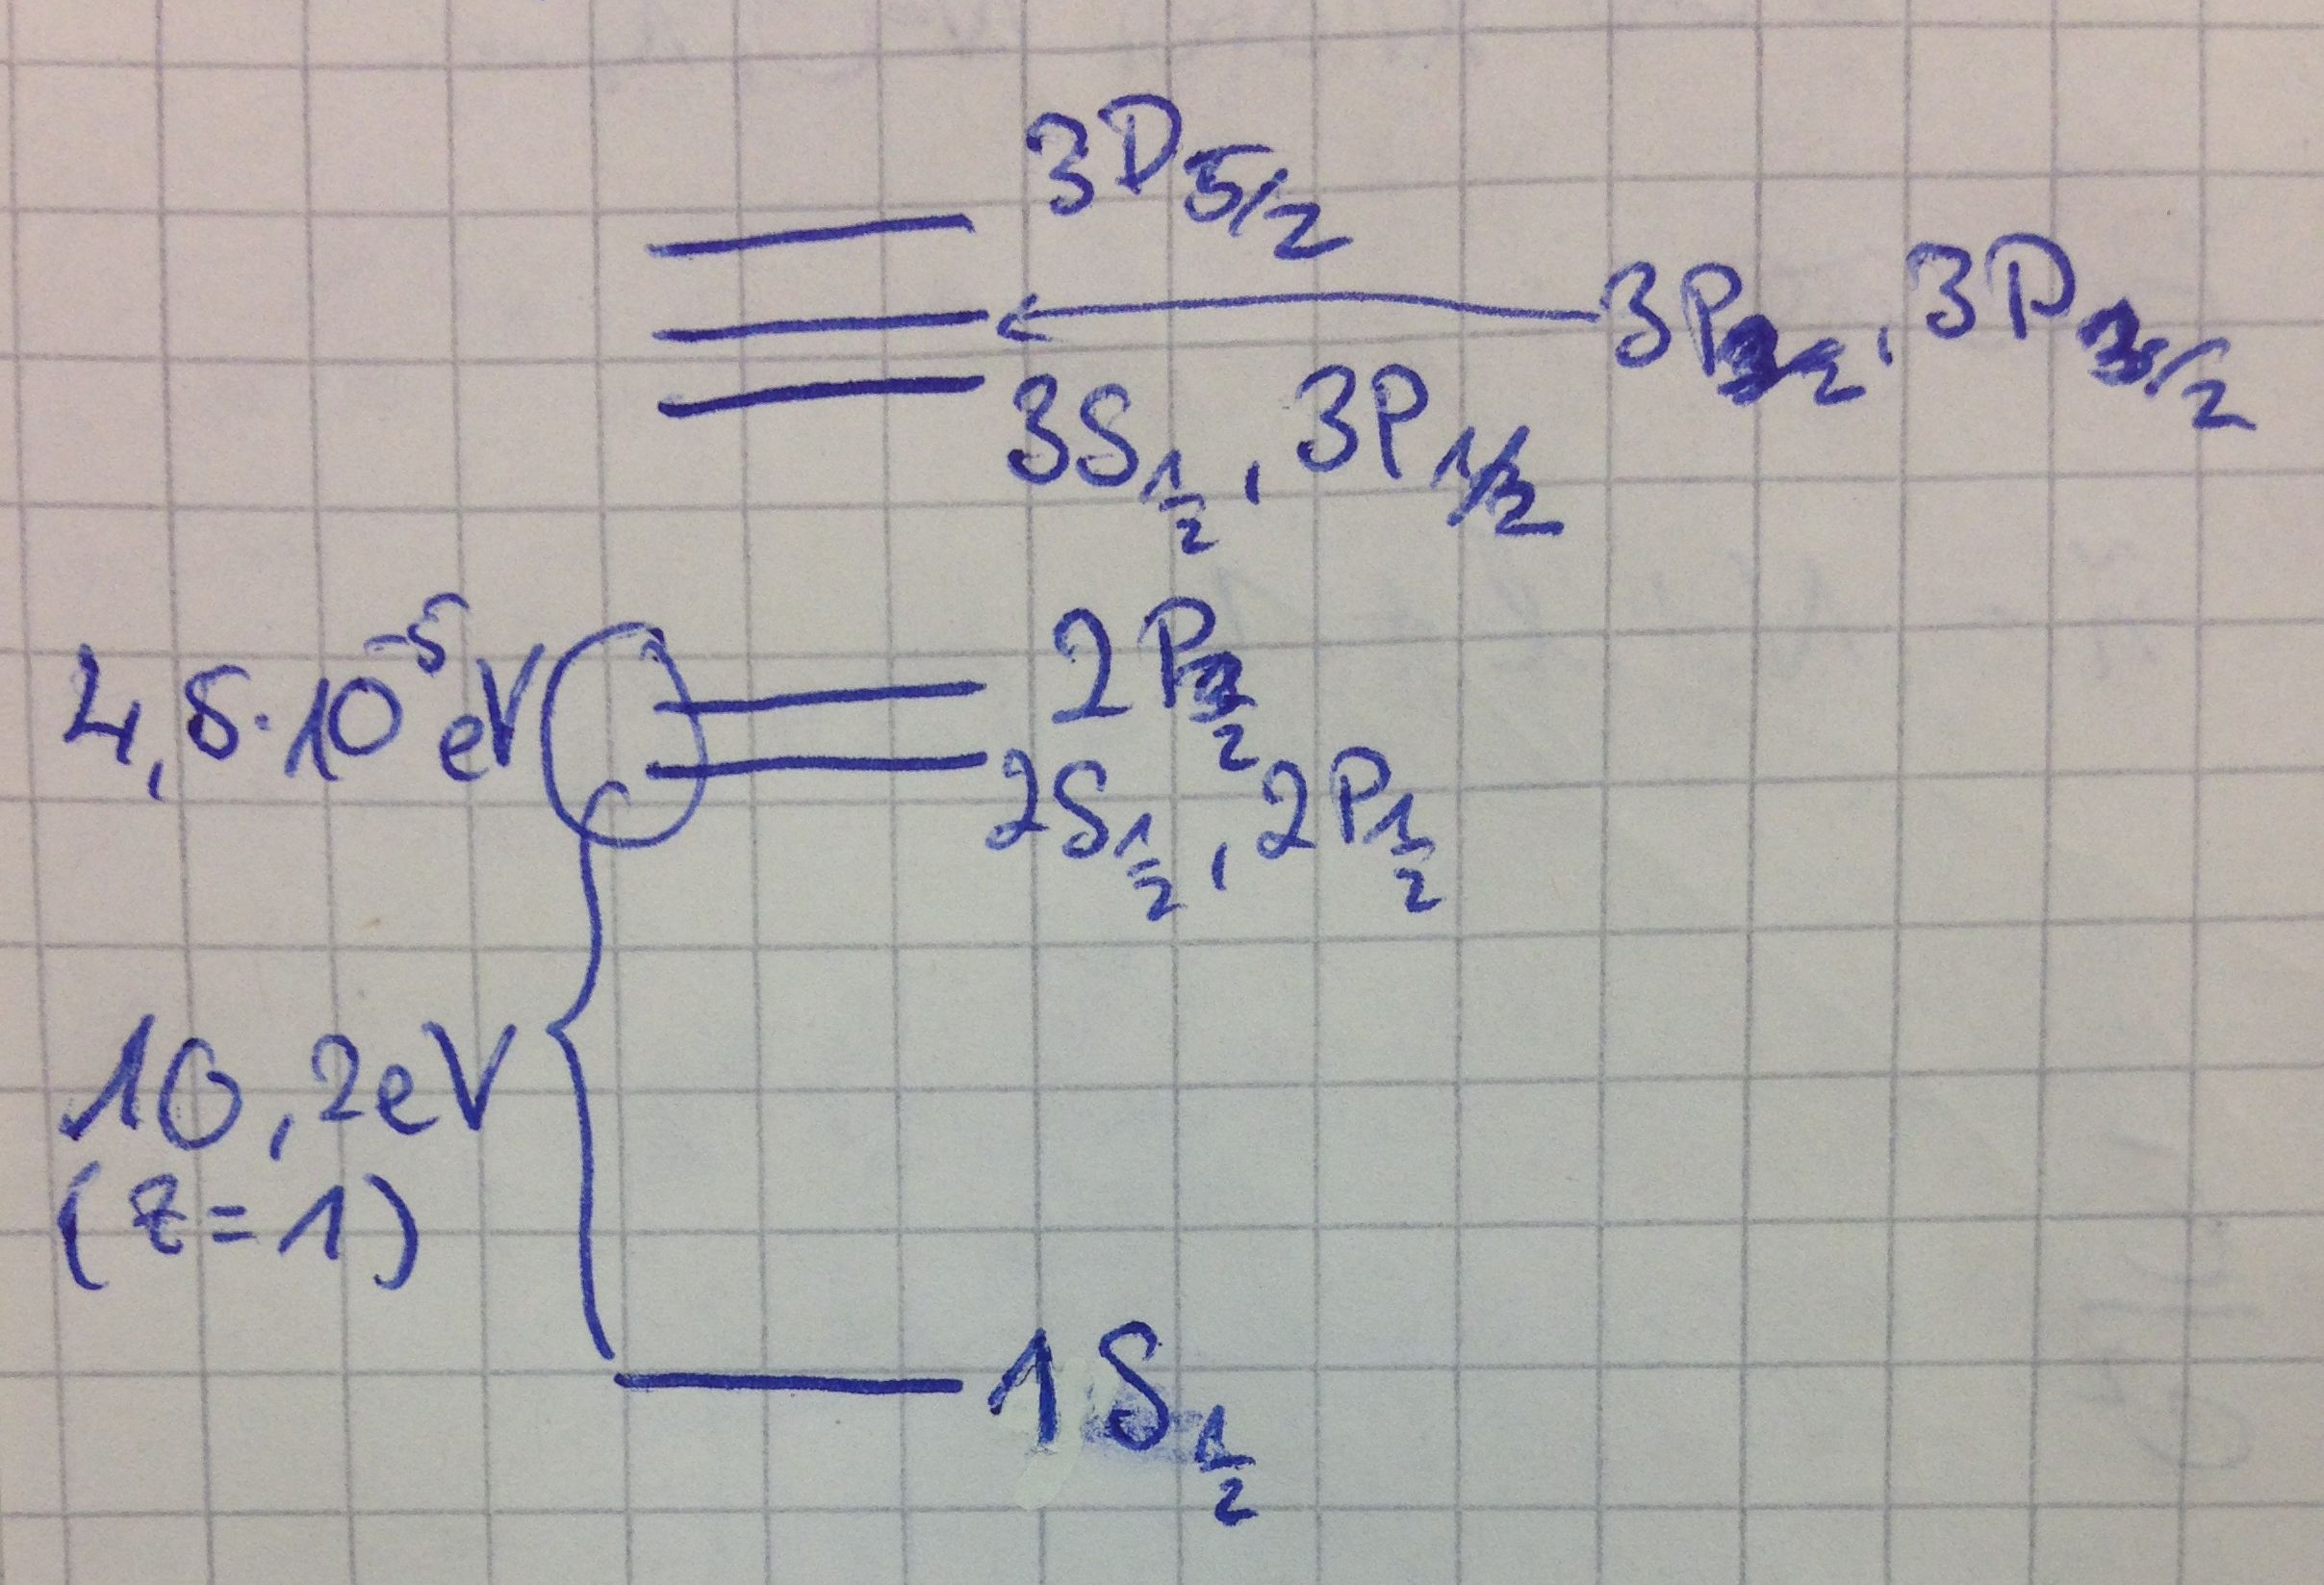
\includegraphics[width=10cm]{Relativistisches_Coulombproblem1}
		\end{center}
	\end{figure*}
Die $j$-Entartung wird beim realistischen Problem aufgehoben durch:
	\begin{itemize}
		\item Wechselwirkung mit magnetischem Moment des Atomkerns: \\
			(Hyperfeinstruktur)
			$\sim 5,8 \cdot 10^{-6} e$V für $ H:~ ^1S_{\frac{1}{2}} \sim \frac{1}{n^2}$ 
		\item Endliche Kernausdehnung 
			$\sim -\frac{1}{n^3} $ für $ H:~ 4\cdot 10^{-1} e$V
		\item Lambshift für $H:~ ^2S_{\frac{1}{2}} / ^2P_{\frac{1}{2}}: ~ 
		4,3 \cdot 10^{-6} e$V \\
			(Effekt des quantisierten elektromagnetischen Feldes, QED)
	\end{itemize}
Problem bei $Z\sim \frac{1}{\alpha} \sim 137$
\\
Konsistene Beschreibung hochionisierter Groß-$Z$-Atome ist nicht im Rahmen einer 1-Teilchen-Theorie möglich (Erzeugung viertueller $e^+e^-$-Paare $\Rightarrow$ QED)